\section{On Unsatisfiable Cores of Ideals with Empty Variety}

Consider the polynomial ring $\Fkk[x_1, \dots, x_n]$, and an ideal $J$
generated by a set of polynomials $F = \{f_1, \dots, f_s\},
\idealj$. Suppose that it is known that $V(J) = \emptyset$, or
otherwise it is determined so by applying the Gr\"obner basis
algorithm. Throughout this document, we will assume that the set $F$
is such that $V(f_1, \dots, f_s) = \emptyset$, unless stated
otherwise. An interesting (and important) problem to solve is as
follows:   

\begin{Problem}
Identify a subset of polynomials $F_c \subseteq F, J_c = \langle F_c
\rangle$, such that $V(J_c) = \emptyset$ too. For lack of a better
term, let us call $F_c$ the infeasible core or the unsatisfiable
core (UNSAT core) of $F$. The terminology is borrowed from the domain of
Boolean Satisfiability solvers. If you can think of a better
terminology, please let me know. 
%Here $F_c = \{f_i : f_i \in F, i\leq s\}$.
\end{Problem}

UNSAT cores have important uses in post-verification debugging, and in
many abstraction-and-refinement techniques used in the analysis of
circuits and systems. Any contribution here will be important. 

\begin{Example}\label{ex1}
Consider the following set of polynomials:
\begin{align*}
f_1: & ab\\
f_2: & ab+a\\
f_3: & ab+b\\
f_4: & ab+a+b+1\\
f_5: & xy+y+x+1\\
f_6: & yz+y+z+1\\
f_7: & c + d\\
f_8: & c + d + 1
\end{align*}

Let $F = \{f_1, \dots, f_8\}$ and $J = \langle F \rangle \subseteq
\F_2[a, b, c, d, x, y]$ where $\F_2 = \{0, 1\}$. Then
$V_{\overline{\F_2}}(J) = \emptyset$ as $GB(J) = \{1\}$. 

Now consider the subset $F_c = \{f_1, \dots, f_4\}, J_c = \langle
F_c\rangle$; it turns out that $V_{\overline{\F_2}}(J)= \emptyset$ as
well, so $F_c$ is an UNSAT core of $F$. Likewise, $\{f_7, f_8\}$ also
form a core. 
\end{Example}


Any set of polynomials $F$ with empty variety is an UNSAT core in
itself. There may be more than one UNSAT cores in $F$, some
polynomials may or may not be common to multiple cores (i.e. these
cores may be non-disjoint), and these cores may have
different cardinalities (different $|F_c|$). The UNSAT core problems
are therefore further classified as: 
\bi
\item Identify a {\it minimum} core, i.e. a core of minimum
  cardinality. In Ex. \ref{ex1}, the set $\{f_7, f_8\}$ is a minimum
  core. [Hardest problem to solve?]
\item Identify a {\it minimal} core. An UNSAT core $F_{c}$ is minimal
  with respect to the property that while the variety of $F_{c}$ is
  empty, the variety of {\it any} subset of $F_c$ is {\it non-empty},
  i.e. $V( F_{c} - \{f_i\} ) \neq \emptyset$ for any $f_i \in
  F_c$. The set $\{f_1, \dots, f_4\}$ constitutes a minimal
  core. [Very important problem, but I guess still a Hard Problem to
    solve!] 
\item Identify any UNSAT core disregarding minimality; i.e. find any
  subset $F_c$ of $F$. For very large problems, sometimes it is
  beneficial to solve this problem, so long as we can experimentally
  demonstrate that the obtained cores are small and their size is close to
  minimal cores --- but maybe algorithmically they can be found very
  quickly/efficiently, whereas finding minimal/minimum cores may be
  computationally infeasible. 
\ei


\begin{Conjecture}
Buchberger's algorithm, and only 1 iteration of it, could be used to
identify a {\it minimal} core. 
\end{Conjecture}

\begin{Conjecture}
Buchberger's algorithm may also be used to identify a {\it minimum}
core, but it will probably require the enumeration of all cores. 
\end{Conjecture}

So,
let us ignore the {\bf minimum} core problem for now, and concentrate
on the {\bf minimal} one. 

The UNSAT core problem should be related to Gr\"obner bases. Suppose
that we are given $F_c = F - \{f_j\}$. Then, if $GB(F) = \{1\}$ and if
$GB(F_c) = \{1\}$ too, then doesn't it imply that $f_j \in \langle F_c
\rangle$? My reasoning is as follows: Denote $J = \langle F \rangle,
J_c = \langle F_c \rangle$. Since $V(J) = V(J_c) = \emptyset$, from
the Weak Nullstellensatz we have $J = J_c = \Fkk[x_1, \dots,
  x_n]$. This implies that $f_j$ can be composed of polynomials of
$F_c$, or $f_j \in F_c$. So $f_j$ is not part of the UNSAT core and
that can be identified using Gr\"obner bases. [Florian: Do you have a
  better/cleaner argument for this?]

\section{Investigating Algorithms to find UNSAT cores $F_c$ from $F$}

A n\"aive way (and inefficient way) to identify {\it a minimal core}
using the GB computation is given in Algorithm 1. In the algorithm, we
pick a polynomial $f_i$ and see if $V(F_c - \{f_i\}) = \emptyset$
(i.e. $F_c - \{f_i\}$ is also infeasible/UNSAT). If so, discard $f_i$
from the core; otherwise keep $f_i$ in the 
core. Pick a different $f_i$ and continue until all polynomials $f_i$
are visited. This algorithm {\it will produce a minimal core}, as we
have tested each polynomial $f_i$ for inclusion in the core. This
requires $O(|F|)$ calls to the GB engine, which is really impractical. 



\begin{algorithm}[hbt]
\caption{Find a minimal UNSAT core}\label{alg:MUS}
\label{alg1}
\begin{algorithmic}

 \REQUIRE{$F=\{f_1,\dots,f_s$\}, $J = \langle F \rangle$ } 
 \ENSURE{The minimal core $F_c \subset F$}
  %%%%%%%%%%%%%%%%%%%%
 \STATE{/* First of all, set $F$ as the core itself*/\;}
 \STATE{$F_c \gets F$;} 

 \FORALL{$f_i \in F_c$}
   \IF{ $\text{Gr\"obnerBasis}(F_c - \{f_i\}) = \{1\}$ } 
     \STATE{/* Discard polynomial $f_i$ as it does not belong to the core*/\;}
     \STATE{$F_c \leftarrow F_c - \{f_i\}$\;}
   \ELSE 
     \STATE{ Keep $f_i$ in the minimal core\;}
   \ENDIF
 \ENDFOR
 \RETURN {$F_c$ as the core}
\end{algorithmic}
\end{algorithm}


The question is if we can identify a core by analyzing the
$Spoly(f_i,f_j)\xrightarrow{F}_+1$ computation itself? Note here
that since $F$ is an UNSAT core, there definitely exists one iteration
of Buchberger's algorithm where $Spoly(f_i, f_j) \xrightarrow{F}_+ 1$
is achieved. We think that a core can definitely be found, and we will
show you how. Then we need to investigate further whether our approach
can be used to identify minimal cores without invoking the GB engine
multiple times. 

Recall that each step of division $f \xrightarrow{f_i}_+r$ operates as
$r = f - \frac{lt(f)}{lt(f_i)} f_i$. If $f$ is to be divided by (say)
two polynomials $f_i, f_j$, then: i) first we see if $lt(f_i) ~|~
lt(f)$. If so, then $lt(f)$ is canceled by $lt(f_i)$. ii) Otherwise,
we check to see if $lt(f_j)$ cancels $lt(f)$. This implies that while
performing the division $f \xrightarrow{f_1, \dots, f_s}_+r$, we can
identify (or keep track of) which polynomials in $f_1, \dots, f_s$ are
used to cancel terms of $f$. 

I will demonstrate the core identification with an Example.

\begin{Example}
Consider the set $F = \{f_1, \dots, f_8\}$ given in Ex
\ref{ex1}. Assume that our term order is LEX with $a > b > c > d > x >
y$.  Apply Buchberger's algorithm to $F$. 

\ben
\item Suppose that in the first
iteration $Spoly(f_1, f_4) \xrightarrow{F}_+r_1$ is computed. 
$Spoly(f_1, f_4) = a+b+1 = r_1$. Mark $f_1, f_2$ and keep them in the
set $F_m = \{f_1, f_4\}$. Since no polynomial
in $F$ divides $r_1$, we have $Spoly(f_1, f_4) \xrightarrow{F}_+ r_1 =
a+b+1$. No other polynomials (divisors) are marked. 

\item Update $F = F \cup r_1$

\item In the next iteration of Buchberger's algorithm, suppose we pair
  $r_1$ with $f_4$, and obtain  $Spoly(r_1, f_4)  = a + b^2 +
  1$. Polynomial $a+b^2+1$ is divisible by $r_1$, so $Spoly(r_1,
  f_4)\xrightarrow{F}_+r_2$, where $r_2 = b^2 + b$. Since $r_1$ is not
  a polynomial from the original set (it is derived from $f_1, f_4$),
  it is not marked. Update $F = F \cup r_2$, and the set of marked
  polynomials is still $F_m = \{f_1, f_4\}$.

\item Let us draw a graph representing this sequence of
  computations. This is shown in Fig. \ref{fig:trace} (a). The
  vertices (nodes) in the graph represent polynomials (marked or
  unmarked). Every vertex (polynomial) has either 0 or 2 incoming
  edges representing the $Spoly$ pair that derived it. It may also
  represent the remainder obtained from the dividend and the divisor
  (e.g. $a+b^2+1 \xrightarrow{a+b+1}_+ b^2+b$). [This graph is just to
    illustrate a book-keeping procedure].

\item We continue: Suppose that Buchberger's algorithm picks
  $S(f_1, f_2)  = a$. Now $r_1$ divides $a$, so $S(f_1, f_2)
  \xrightarrow{r_1}_+ r_3 = b+1$. $F = \{f_1, \dots, f_8, r_1, r_2,
  r_3\}$. Mark $f_1, f_2$ so that $F_m = \{f_1, f_4, f_2\}$. 
\item Next, $Spoly(f_1, f_3) = b$, and $b\xrightarrow{r_3}_+1$. Bingo!
  Mark $f_1, f_3$, $F_m = \{f1, \dots, f_4\}$.  Note that  $r_3$ is not marked as
  it is a derived polynomial. 

\item Update the graph, as  shown in Fig. \ref{fig:trace} (b).


\item Now, starting from the \textbf{1} node, traverse the graph
  backwards, to reach/identify all the vertices that are sources,
  i.e. those that have no incoming edges. Clearly, vertices 1, 2, 3, 4
  are the source vertices in this case. Of these vertices, identify
  only those that are marked in $F_m$. In this special case, all 4 of
  them are marked; so the core is obtained as $F_c = F_m$; in general, 
  we would only chose the marked vertices in the core. 

\item Just for fun, and to prove a point, compute $S(f_5, f_6)
  \xrightarrow{F}_+0$, so nothing is added to the Spoly graph. On the
  other hand, $Spoly(f_7, f_8)$ would have given us the   minimum
  core. 
\een

\end{Example}



\begin{figure}[hbt]
\centering
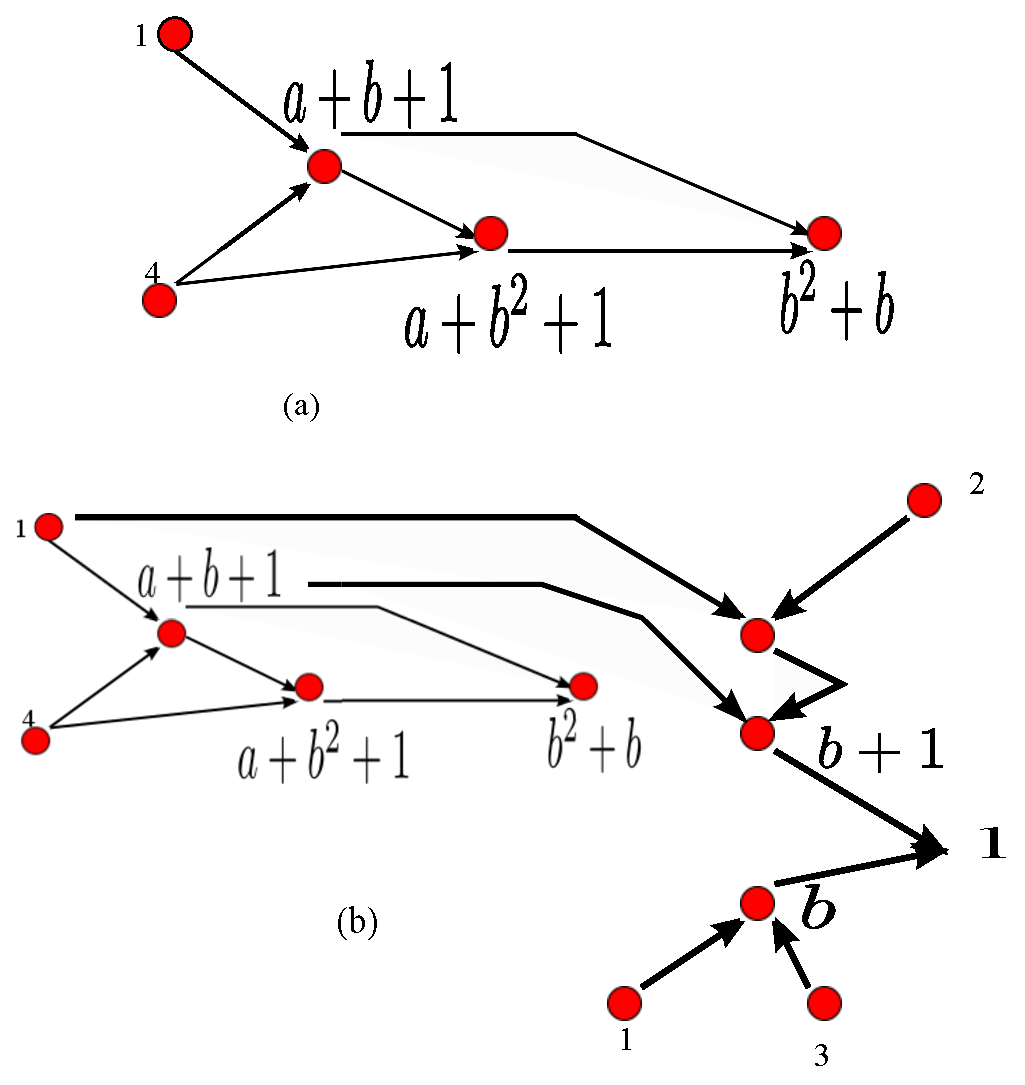
\includegraphics[scale=0.6]{trace.eps}
\caption{Keeping track of polynomials involved in $GB(J) = \{1\}$}
\label{fig:trace}
\end{figure}

Coming to the point: i) Keep track of all $Spoly(f_i,
f_j)\xrightarrow{f_1, \dots, f_s}_+ r$; ii) mark $f_i, f_j$ if $r\neq
0$; iii) Mark those $f_l$'s that have leading terms that cancel
monomial terms in $Spoly(f_i, f_j)$; iv) Build this Spoly graph (I
don't yet have a catchy name for this graph); v) Once $1\in J$ is
detected, traverse the graph to identify all the marked polynomials that were
used in obtaining this unit element. These polynomials constitute the
core.

\begin{Problem}
Does the approach guarantee a minimal core? If yes, how do we show it?
If not, we need to generate an example to understand it better. The
example that I have derived is too trivial. Probably we need to find
more complicated examples to test the idea. 
\end{Problem}

Questions and comments are welcome. 

%% Clauses:
%% \begin{align*}
%% \bar{a}\lor\bar{b}\\
%% a\lor\bar{b}\\
%% \bar{a}\lor b\\
%% a\lor b\\
%% x\lor y\\
%% y\lor z
%% \end{align*}

